\documentclass{article}

\usepackage{units} 
\usepackage{graphicx}
\usepackage[fleqn]{amsmath}
\usepackage{cancel}
\usepackage{float}
\usepackage{mdwlist}
\usepackage{booktabs}
\usepackage{cancel}
\usepackage{polynom}
\usepackage{caption}
\usepackage{fullpage}
\usepackage{xfrac}
\usepackage{enumerate}

\newcommand{\degree}{\ensuremath{^\circ}} 
\everymath{\displaystyle}

% \begin{figure}[H]
%   \centering
%   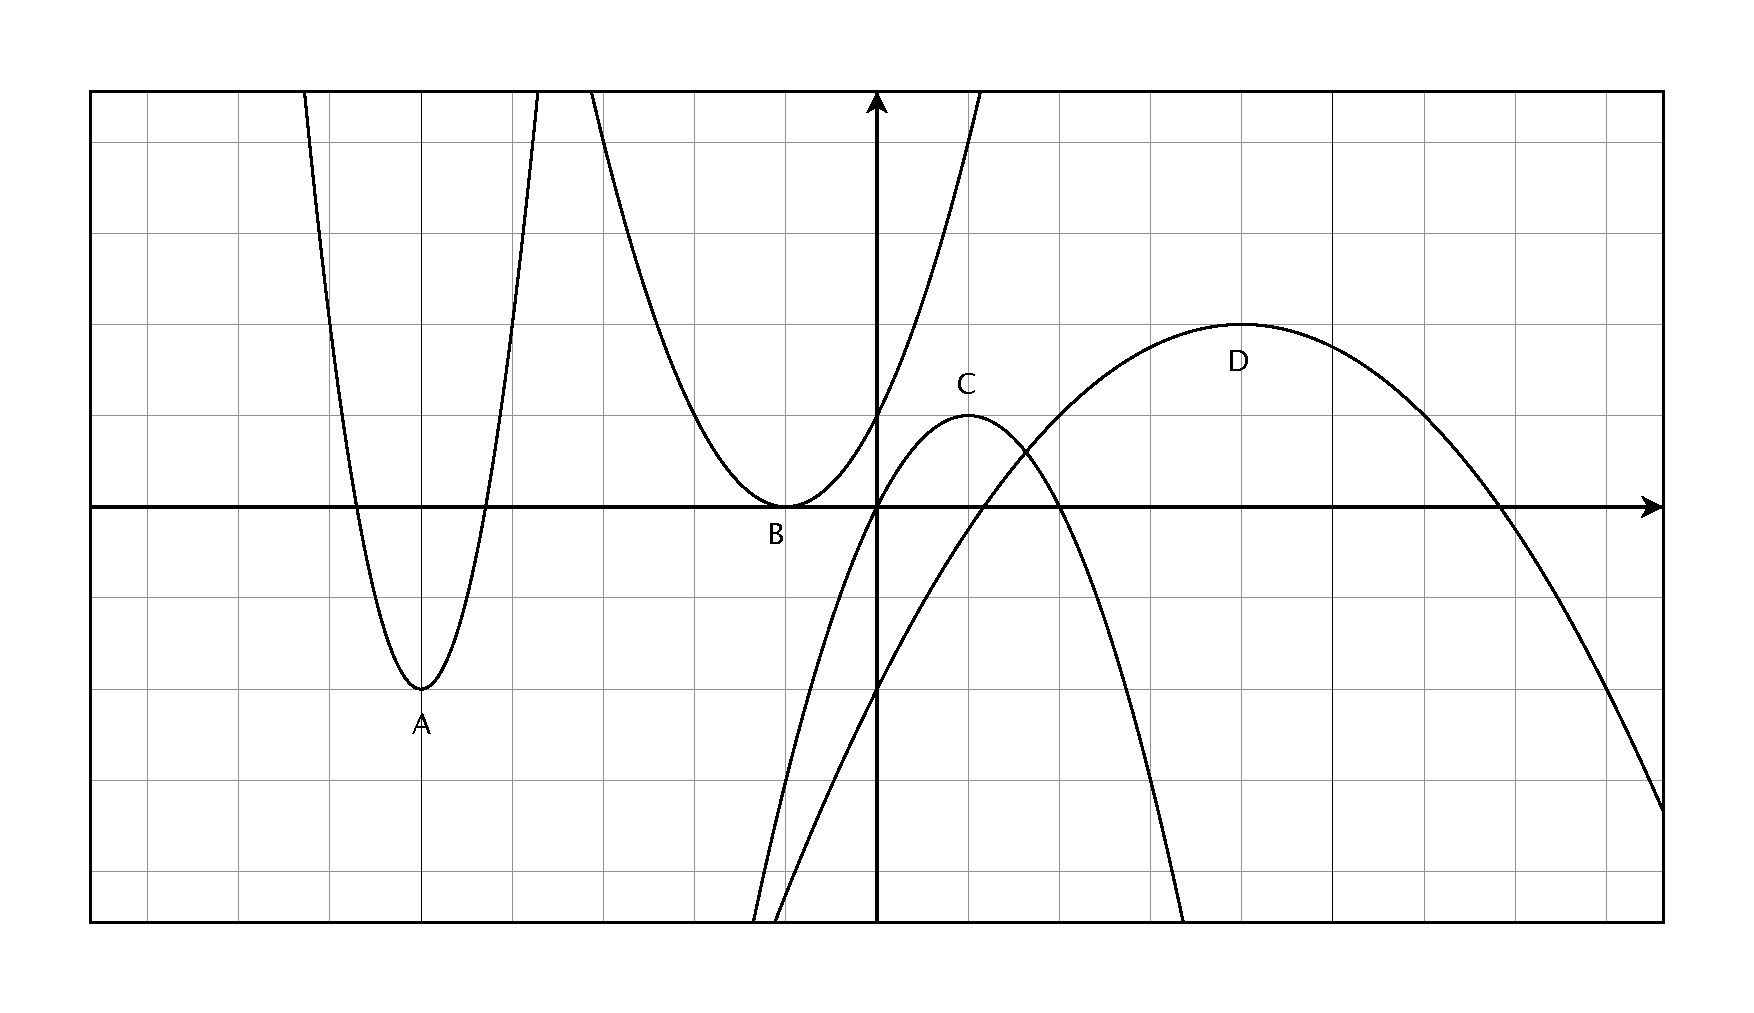
\includegraphics[scale=.3]{problem_7.eps}
%   \caption*{Problem 7}
% \end{figure}

% \begin{tabular}{cc}
% \toprule
% period & amplitude \\
% \midrule
%   $\pi$ & $2$ \\
% \bottomrule
% \end{tabular}

\title{Math 141 Notes \\ Section 3.1}
\date{March 27, 2013}

\begin{document}

\maketitle
\tableofcontents

\section{Polynomials}

\subsection{Definitions}

\begin{itemize*}
  \item A polynomial is an expression that only contains +, -, and integer powers of $x$.
  \item The {\em degree} is the largest exponent.
  \item The {\em leading coefficient} is the coefficient of the term with the largest exponent.
  \item The {\em constant coefficient} is the coefficient without an $x$.
\end{itemize*}

\subsection{Zeros}
For polynomial $P$ and real number $c$, the following statements are equivalent:
\begin{itemize*}
  \item $c$ is a zero of $P$
  \item $x = c$ is a solution to $P(x) = 0$
  \item $x - c$ is a factor of $P(x)$
  \item $x = c$ is an x-intercept of the graph of $P(x)$
\end{itemize*}

\subsection{Intermediate Value Theorem}
If $P(a)$ and $P(b)$ have opposite signs, then there is at least one value, $c$ between $a$ and $b$ where $P(c) = 0$.

\section{Polynomial Graphs}
\subsection{Appearance}

\begin{itemize*}
  \item Graphs of polynomials are always continuous and smooth.
  \item The higher the degree the more bumps might be present.
  \item Graphs of odd-degree polynomials always look generally like the graph of $y = x^3$
  \item Graphs of even-degree polynomials always look generally like the graph of $y = x^2$
  \item For ``large'' values of $x$, only the leading coefficient matters
\end{itemize*}

\subsection{End Behavior}
\begin{itemize*}
  \item The behavior for ``large'' or ``small'' values of $x$ is the ``end behavior''
  \item The end behavior only depends on the highest degree term.  The four cases are:
    \begin{itemize*}
      \item Even degree and positive leading coefficient
      \item Even degree and positive leading coefficient
      \item Odd degree and negative leading coefficient
      \item Odd degree and negative leading coefficient
    \end{itemize*}
\end{itemize*}

\subsection{Effect of Multiplicity of Zeros}
\begin{itemize*}
  \item For zeros of multiplicity 1, the graph just crosses the x-axis
  \item For zeros of even multiplicity, the graph touches the x-axis and changes direction
  \item For zeros of odd multiplicity greater than 1, the graph flattens out at the x-axis and keeps going
\end{itemize*}

\begin{figure}[H]
  \centering
  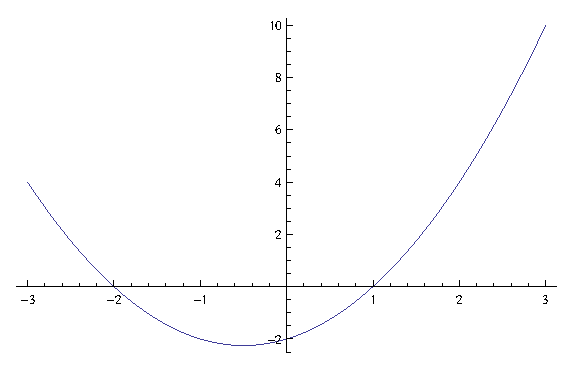
\includegraphics[scale=0.9]{graph2.eps}
  \caption*{Multiplicity One: $P(x) = x^2 + x - 2 = (x - 1)(x + 2)$}
\end{figure}

\begin{figure}[H]
  \centering
  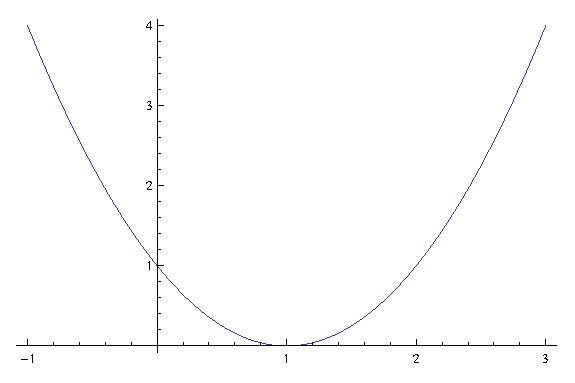
\includegraphics[scale=0.9]{graph1.eps}
  \caption*{Even Multiplicity: $P(x) = (x - 1)^2$}
\end{figure}

\begin{figure}[H]
  \centering
  
\includegraphics[scale=0.9]{graph3.eps}
  \caption*{Odd Multiplicity: $P(x) = (x - 1)^3$}
\end{figure}

\subsection{Local Extrema}
A polynomial of degree $n$ has at most $n - 1$ local extrema.  
\begin{itemize*}
  \item A parabola (degree 2) has one local extreme
  \item $f(x) = x^3$ has no local extrema
  \item $f(x) = x^3 + x^2 - 2x = x(x - 1)(x + 2)$ has two local extrema
\end{itemize*}

\begin{figure}[H]
  \centering
  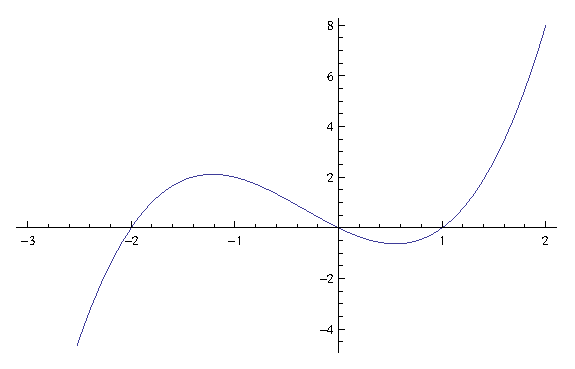
\includegraphics[scale=0.9]{graph4.eps}
  \caption*{Local Extrema: $P(x) = x^3 + x^2 - 2x$}
\end{figure}

\section{Graphing Problems}
\subsection{Procedure}

\begin{itemize*}
  \item Factor to find zeros
  \item Check multiplicity
  \item Find the end behavior
  \item Try a few sample points between the zeros
  \item Graph
\end{itemize*}

\subsection{Examples}
\begin{enumerate}
  \item 
    \begin{align*}
      f(x) &= x^3 + x^2 - 2x \\
           &= x(x + 2)(x - 1)
      \\
      x    &= \left\{ -2, 0, 1 \right\} \\
    \end{align*}
    
    \begin{figure}[H]
      \centering
      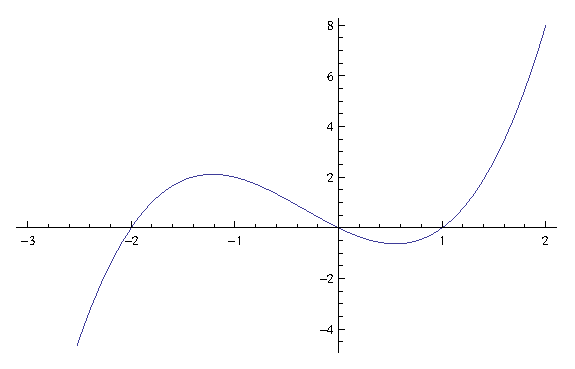
\includegraphics[scale=0.9]{graph5.eps}
      \caption*{$f(x) = x^3 + x^2 - 2x$}
    \end{figure}

  \item 
    \begin{align*}
      f(x) &= (x + 2)^2(x - 3) \\
      \\
      x    &= \left\{ -2, 3 \right\} \\
    \end{align*}
    
    \begin{figure}[H]
      \centering
      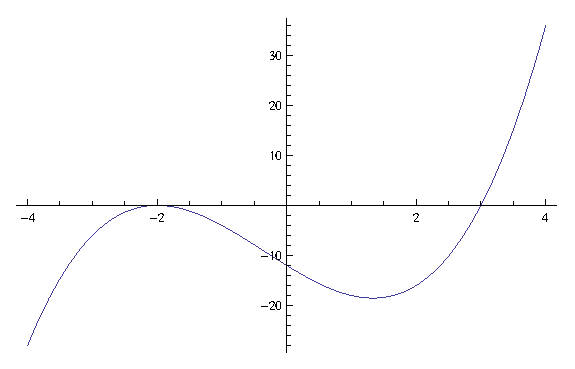
\includegraphics[scale=0.9]{graph8.eps}
      \caption*{$f(x) = (x + 2)^2(x - 3)$}
    \end{figure}

  \item 
    \begin{align*}
      f(x) &= (x - 1)^2 (x + 2)^2 \\
      \\
      x    &= \left\{ -2, 1 \right\} \\
    \end{align*}
    
    \begin{figure}[H]
      \centering
      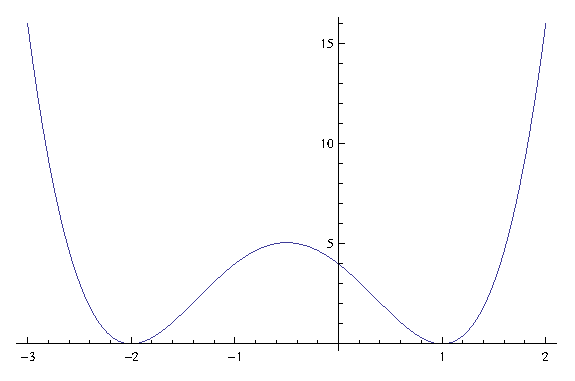
\includegraphics[scale=0.9]{graph9.eps}
      \caption*{$f(x) = (x - 1)^2 (x + 2)^2$}
    \end{figure}

  \item 
    \begin{align*}
      f(x) &= (x - 1)^3 (x + 2) \\
      \\
      x    &= \left\{ -2, 1 \right\} \\
    \end{align*}
    
    \begin{figure}[H]
      \centering
      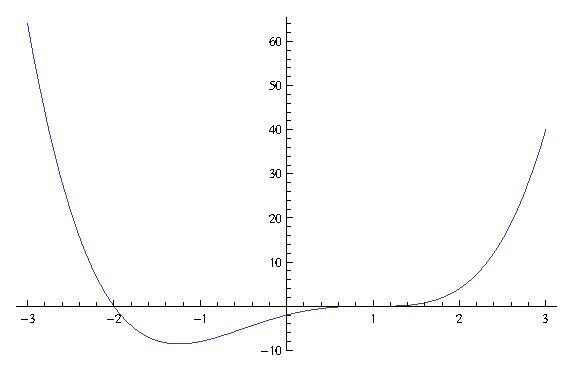
\includegraphics[scale=0.9]{graph11.eps}
      \caption*{$f(x) = (x - 1)^3 (x + 2)$}
    \end{figure}


  \item 
    \begin{align*}
      f(x) &= x^3 + x^2 - 4x - 4 \\
           &= x^2(x + 1) - 4(x + 1) \\
           &= (x^2 - 4)(x + 1) \\
           &= (x + 2)(x - 2)(x + 1) \\
      \\
      x    &= \left\{ -2, -1, 2 \right\} \\
    \end{align*}
    
    \begin{figure}[H]
      \centering
      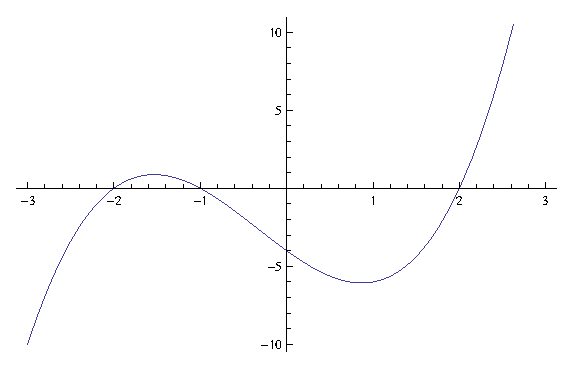
\includegraphics[scale=0.9]{graph6.eps}
      \caption*{$f(x) = x^3 + x^2 - 4x - 4$}
    \end{figure}

  \item 
    \begin{align*}
      f(x) &= 2x^3 + x^2 - 2x - 1  \\
           &= x^2(2x + 1) - (2x + 1) \\
           &= (x^2 - 1)(2x + 1) \\
           &= (x + 1)(x - 1)(2x + 1) \\
      \\
      x    &= \left\{ -1, - \frac{1}{2}, 1 \right\}
    \end{align*}
    
    \begin{figure}[H]
      \centering
      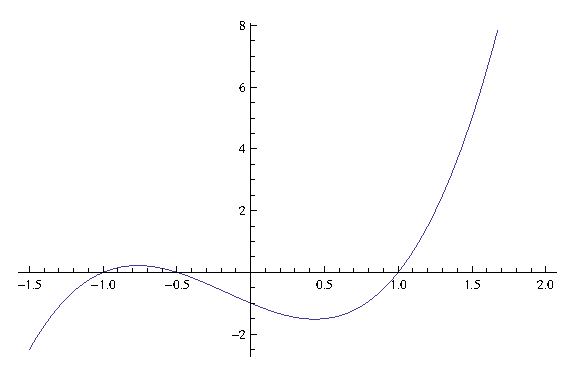
\includegraphics[scale=0.8]{graph7.eps}
      \caption*{$f(x) = 2x^3 + x^2 - 2x - 1$}
    \end{figure}

  \item 
    \begin{align*}
      f(x) &= x^4 - 10x^2 + 9 \\
           &= (x^2 - 9)(x^2 - 1) \\
           &= (x + 1)(x - 1)(x + 3)(x - 3) \\
      \\
      x    &= \left\{ \pm 3, \pm 1 \right\}
    \end{align*}
    
    \begin{figure}[H]
      \centering
      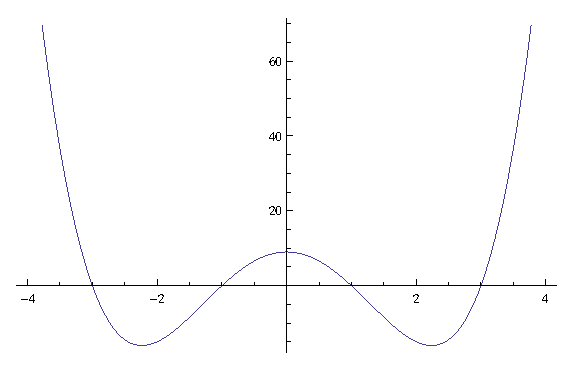
\includegraphics[scale=0.9]{graph10.eps}
      \caption*{$f(x) = x^4 - 10x^2 + 9$}
    \end{figure}

\end{enumerate}

\end{document}
